\subsection{Feature Competition Within Token Preferences}

We now fix the target type and inspect which shared readout features carry the
positive and negative terms in low-error logit differences.

\paragraph{From preferences to features.}
Logit differences expose feature competition compressed by top-token lens
summaries. In \Cref{fig:main-lens-prism-comparison}, a
\texttt{verify}-versus-\texttt{assume} preference becomes signed SRP feature
terms with explicit reconstruction error.

\paragraph{Polysemous-token local score accounts.}
For the main case studies, we apply SRP to low-error Qwen3.5-2B polysemous-token
logit differences in \Cref{fig:selected-readout-prism-examples}. In an insect
context, \texttt{bug} draws on mosquito, bee, and beetle features against
error-token features; in software, it draws on defect, crash, and debug
features. The two \(32\times\), \(k=256\) panels have relative reconstruction
errors \(0.185\) and \(0.003\). Additional \texttt{bark} and \texttt{bass}
cases, plotting conventions, and label audits appear in
\cref{fig:app-selected-readout-prism-extra-examples,app:display-taxonomy,tab:app-main-case-study-feature-audit}.
These sign-preserved, low-\(\rho\) examples show target-local support: the same
surface token can be supported by different feature families as the competing
alternative and context change; aggregate frequencies are in the tables.

\begin{figure}[H]
    \centering
    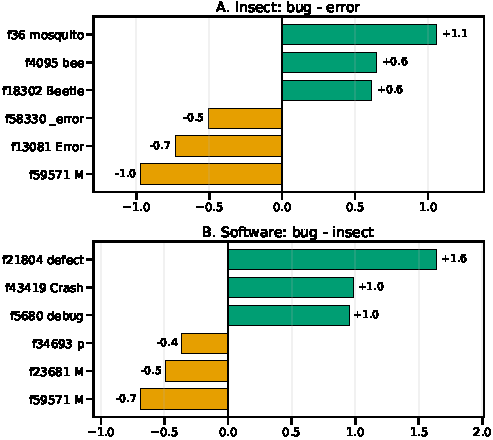
\includegraphics[width=0.86\columnwidth]{figures/proto_token_lens/qwen2b_32x_section43_polysemy_margin_curated_examples/qwen2b_32x_margin_examples_main2_onecol_with_tokens.pdf}
    \caption{\textbf{Sparse Readout Prism case studies.}
    Positive/negative bars support the first/second token; the axis is signed
    contribution. Relative reconstruction errors are \(0.185\) and \(0.003\).
    Both panels use the selected Qwen3.5-2B unembedding-row SAE
    (\(D=65536\), \(k=256\)); feature names come from highest-activating rows;
    see \cref{tab:app-main-case-study-feature-audit}.}
    \label{fig:selected-readout-prism-examples}
\end{figure}
